\chapter{Bass-Serre-Theorie}

% =============
\section{Die Fundamentalgruppe eines Graphen}\label{sec_FG}

\DB Es sei $\GR$ ein zusammenhängender Graph und $p\in E(\GR)$.
\begin{enumerate}
\item $\pi_1(\GR,p)$ sei die Menge der stachelfreien geschlossenen
Wege in $\GR$ mit Anfangs- und Endpunkt $p$.
\item Für $w_1, w_2\in \pi_1(\GR,p)$ sei $w_1\cdot w_2$ der
Weg, den man nach dem Entfernen aller Stachel des aus $w_1$ und $w_2$
zusammengesetzen Weges erhält.
\item Mit dieser Verknüpfung ist $\pi_1(\GR,p)$ eine Gruppe.
Sie heißt \emph{Fundamentalgruppe}\index{Fundamentalgruppe}\index{Gruppe!Fundamental-}\index{$\pi_1(\GR,p)$, $\pi_1(\GR)$}
von $\GR$ (bzgl. $p$).
\item Für jedes $q\in E(\GR)$ ist $\pi_1(\GR,q)\cong\pi_1(\GR,p)$.
Daher können wir auch $\pi_1(\GR)$ schreiben.
\end{enumerate}
\bew
\begin{itemize}
\item[3.] Das neutrale Element ist der Weg der Länge $0$.
Zu $w=(k_1,\ldots,k_n)$ ist
$\bar{w}=(\bar{k}_n,\ldots,\bar{k}_1)$ invers.

Die Zeichnung veranschaulicht, wie beim Zusammensetzen zweier
stachelfreier Wege neue Stachel autreten können.
\begin{center}
	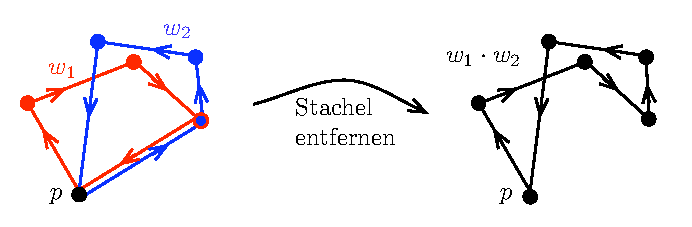
\includegraphics{grugraImages/w1w2}
\end{center}
Hat ein zusammengesetzter Weg $w=(k_1,\ldots,k_n)$ einen Stachel,
so muss $\bar{k}_i=k_{i+1}$ für ein $i$ gelten.
Setze $w^{(1)}:=(k_1,\ldots,k_{i-1},k_{i+2},\ldots,k_n)$ und
wiederholen dieses Vorgehen solange, bis alle Stacheln entfernt sind.
Wir bemerken, dass dies zu einem eindeutigen stachelfreien Weg führt.
Daraus folgt die Wohldefiniertheit der Verknüpfung und ebenso die
Assoziativität.
\item[4.] Es sei $v$ ein Weg in $\GR$ von $p$ nach $q$. Dann ist
\[
\phi:\pi_1(\GR,q)\Ra\pi_1(\GR,p),\quad
w\mapsto vw\bar{v}
\]
ein Gruppenhomorphismus, denn
\[
\phi(w_1 w_2) = v w_1 w_2 \bar{v}
=v w_1 \bar{v} v w_2 \bar{v}
=\phi(w_1)\phi(w_2).
\]
Da es offensichtlich eine Umkehrung gibt, ist $\phi$ bijektiv.
\qed
\end{itemize}

\BSP\
\begin{enumerate}
\item Ist $\GR$ ein Baum, so ist $\pi_1(\GR,p)=\{1\}$.
\item Es sei
\begin{center}
	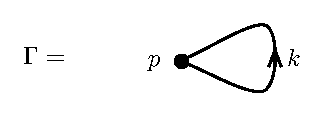
\includegraphics{grugraImages/pi1Z}
\end{center}
Die Gruppe $\pi_1(\GR,p)$ besteht aus dem Weg der Länge $0$
und aus den Wegen, die durch
$n$-faches Durchlaufen von $k$ oder $n$-faches Durchlaufen von
$\bar{k}$ entstehen. Daher ist $\pi_1(\GR,p)\cong\ZZ$.
\item Es sei
\begin{center}
	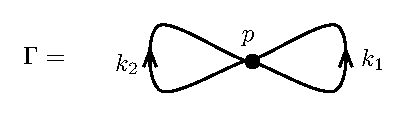
\includegraphics{grugraImages/pi1F2}
\end{center}
In diesem Fall ist $\pi_1(\GR,p)=F_2$.
\end{enumerate}

\PROP\label{prop_zusfrei}
Für jeden zusammenhängende Graphen $\GR$ ist $\pi_1(\GR)$
eine freie Gruppe vom Rang $g(\GR)$.

\bew Für den Fall, dass $\GR$ hat nur eine Ecke hat:\\
Die Kanten $k\in K(\GR)$ können als Elemente von $\pi_1(\GR)$
aufgefasst werden. Für $k\in K(\GR)$ ist $\bar{k}$ das inverse
Element. Die stachelfreien Wege in $\GR$ entsprechen bijektiv
den Kantenfolgen der Form
\[
k_1^{\eps_1},\ldots,k_n^{\eps_n}
\]
mit $n\geq 0$, $\eps_i=\pm 1$ und
$k_{i+1}^{\eps_{i+1}}\neq k_i^{-\eps_i}$.
Diese Stellen aber genau die reduzierten Worte in
$F(K(\GR)^+)$ dar, wobei $K(\GR)^+$ eine Orientierung von
$\GR$ ist.

Nun der Beweis für den allgemeinen Fall:\\
Es sei $T$ ein aufspannender Teilbaum
von $\GR$ und $\GR':=\GR/T$. Nach Bemerkung \ref{bem_GZ}(2) ist
$g(\GR')=g(\GR)$. Zusammen mit dem Fall für eine Ecke genügt es
nun zu zeigen, dass $\pi_1(\GR')\cong\pi_1(\GR)$ ist.
\qed

\BEM Es sei $\GR$ ein zusammenhängender Graph, $Z$ ein Teilgraph
$z\in Z$.
Dann gibt es einen surjektiven Homomorphismus
$\phi_Z:\pi_1(\GR,z)\Ra\pi_1(\GR/Z,Z)$, dessen Kern die
normale Hülle von $\pi_1(Z,z)$ ist, d.h.
\[
\K{\phi_Z}=\lag\pi_1(Z,z)\rag_{\mathrm{NT}}:=
\bigcap_{\pi_1(Z,z)\subset N \unlhd \pi_1(\GR,z)} N.
\]
\bew Für $w=(k_1,\ldots,k_n)\in\pi(\GR,z)$ sei
$\psi_Z(w)$ der Weg, der durch Streichen alle Kanten in $K(Z)$
entsteht und $\phi_Z(w)$ der Weg, der durch Entfernen aller Stacheln
aus $\psi_Z(w)$ entsteht. Man sieht leicht, dass $\phi_Z$ ein
Gruppenhomomorphismus ist.

$\phi_Z$ ist surjektiv: Fasse $w$ als Weg in $\pi_1(\GR/Z,Z)$ auf.
Dann sind $k_1,\ldots,k_n\in K(\GR)\backslash K(Z)$.
Ist $\ter(k_i)\neq \ini(k_{i+1})$ in $E(\GR)$, so ist
$\ter(k_i)=\ini(k_{i+1})=Z$ in $E(\GR/Z)$.
Da $Z$ zusammenhängend ist, gibt es einen Weg $v_i$ in $Z$ mit
$\ini(v_i)=\ter(k_i)$ und $\ter(v_i)=\ini(k_{i+1})$.
Also ist
\[
\tilde{w}=
(v_0,k_1,v_1,\ldots,k_n,v_n) \in \pi_1(\GR,z)
\]
ein Weg in $\GR$ mit $\phi_Z(\tilde{w})=w$
(dabei dürfen die Wege $v_i$ die Länge $0$ haben und bei Bedarf
sei $v_0$ ein Weg in $Z$ von $z$ nach $\ini(k_1)$ und $v_n$ ein
Weg in $Z$ von $\ter(k_n)$ nach $z$).
\begin{center}
	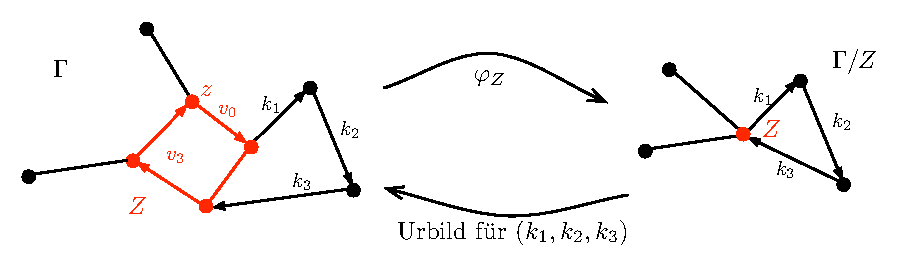
\includegraphics{grugraImages/phiZ}
\end{center}
Offensichtlich liegt $\pi_1(Z,z)$ im Kern von $\phi_Z$. Da der Kern
ein Normalteiler ist, der $\pi_1(Z,z)$ enthält, muss er auch
den Schnitt über alle solchen Normalteiler enthalten,
also $\lag \pi_1(Z,z)\rag_{\mathrm{NT}}\subseteq \K{\phi}$.

Zum Beweis der umgekehrten Inklusionrichtung überlegen wir zuerst,
dass ein Weg $w\in \K{\phi_Z}$ in der Form
\[
v_0 w_1 v_1 w_2 v_2 \cdots w_n v_n
\]
geschrieben werden kann, wobei $v_i$ ein Weg in $Z$ und $w_i$ ein
Weg außerhalb von $Z$ ist (jedoch mit Anfangs und Endpunkt in $Z$).
Es muss $\psi_Z(w)=w_1 w_2 \ldots w_n$ ein Stachel sein.
Wir wählen stachelfreie Wege $u_i\in\pi_1(Z,z)$ von $\ter(w_i)$ nach
$z$ und $u_i'\in\pi_1(Z,z)$ von $\ter(v_i)$ nach $z$.
Dann können wir $w$ schreiben als
\begin{align*}
w &= v_0 w_1 (u_1 u_1^{-1}) v_1 (u_1' u_1'^{-1}) w_2 \cdots \\
&=\ub{v_0 w_1 u_1}{\in \pi_1(\GR,z)}
\ub{u_1^{-1} v_1 u_1'}{\in \pi_1(Z,z)}
\ub{u_1'^{-1} w_1 u_2}{\in \pi_1(\GR,z)} \cdots .
\end{align*}
Wir können also ohne Einschränkung annehmen, dass
$w_i\in\pi_1(\GR,z)$ und $v_i\in\GR(Z,z)$ gilt. Damit erhalten wir
\begin{align*}
w =&
\ub{w_1 v_1 w_1^{-1}}{\lag \pi_1(Z,z)\rag_{\mathrm{NT}}}
\ub{w_1 w_2 v_2 w_2^{-1} w_1^{-1}}{\lag \pi_1(Z,z)\rag_{\mathrm{NT}}}
\ub{w_1 w_2 w_3 v_3 w_3^{-1} w_2^{-1} w_1^{-1}}{\lag \pi_1(Z,z)\rag_{\mathrm{NT}}}\\
&\cdots
\ub{w_1\cdots w_{n-1}\ldots v_1 w_{n-1}^{-1}\cdots w_1^{-1}}{\lag \pi_1(Z,z)\rag_{\mathrm{NT}}}
\cdot
\ub{w_1\cdots w_n}{\text{Stachel}},
\end{align*}
also $w\in\lag \pi_1(Z,z)\rag_{\mathrm{NT}}$.
\qed

\PROP Zu jedem Graphen $\GR$ gibt es einen Baum $X=X_{\GR}$ und eine
freie Aktion von $\pi_1(\GR)$ auf $X$, so dass
$X/\pi_1(\GR)\cong \GR$.

\bew
Es sei $T$ ein maximaler Teilbaum von $\GR$ und $S$ eine Orientierung
von $K(\GR)\backslash K(T)$. Dann ist $\pi_1(\GR)\cong F(S)$
nach Proposition \ref{prop_zusfrei}.

Die Idee, die der folgenden Konstruktion von $X$ zugrunde liegt,
ist es, für jedes Element von $F(S)$ eine Kopie von
$T$ zu erstellen, so dass $F(S)$ frei auf diesen Kopien operieren
kann. Dazu identifizieren wir ein $s\in S$ mit dem Element
von $\pi(\GR)$, dass $s$ enthält und sonst nur Kanten in $T$
(dies ist eindeutig, da $T$ ein Baum ist).
Nun definieren wir $X$ durch
\begin{align*}
E(X) &:= \BCUP{.}{g\in\pi_1(\GR)} g\cdot E(T), \\
K(X) &:= \Bigl(\BCUP{.}{g\in\pi_1(\GR)} g\cdot K(T)\Bigr)
\cup
\Bigl(\BCUP{}{s\in S}\BCUP{}{g\in\pi_1(\GR)} \{gs, g\bar{s} \}\Bigr)
\end{align*}
mit $\ini(gs):=g\ini(s)$, $\ter(gs):=gs\ter(s)$ und entsprechend
für $g\bar{s}$.
$\pi_1(\GR)$ operiert auf $X$ durch Linksmultiplikation.

Es ist $X/\pi_1(\GR)=\GR$ nach Konstruktion. $X$ ist
zusammenhängend, da $S$ die Gruppe $\pi_1(\GR)$ erzeugt
(vgl. Beweis von Proposition \ref{prop_zusfrei}).
Gäbe es Kreise in $X$, so gäbe es ein reduziertes Wort in den
Elementen aus $S$, im Widerspruch dazu, dass die Aktion frei ist.
Somit muss $X$ ein Baum sein.
\qed

\DEF Der Baum $X_{\GR}$ heißt \emph{universelle Überlagerung}\index{universelle Überlagerung} von $\GR$.

\BSP\label{bsp_univ} Es sei
\begin{center}
	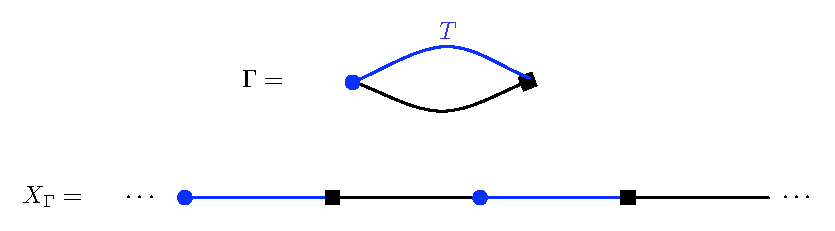
\includegraphics{grugraImages/univ}
\end{center}
$n\in\ZZ=\pi_1(\GR)$ operiert durch Translation um $2n$.

Die hier gegebenen Definitionen der Fundamentalgruppe und der
universellen Überlagerung sind konsistent mit denen aus der
Topologie, wenn wir die Graphen als topologische Teilräume
eines $\RR^n$ auffassen
(vgl. Abschnitte 1.1 und 1.3 in Hatcher \cite{hatcher}).
So entspricht der Graph $\GR$ aus
Beispiel \ref{bsp_univ} dem Einheitskreis $S^1$, dessen
universelle Überlagerung $X_{\GR}$ die reellen Zahlen $\RR$ sind.


% ==================
\section{Freie Produkte und Amalgame}\label{sec_amal}


Es sei $G$ eine Gruppe und $S$ eine Erzeugermenge von $G$.
Die UAE der freien Gruppen impliziert
$G\cong F(S)/\K{\Phi}$ für den Homomorphismus
$\Phi:F(S)\Ra G$, $s\mapsto s$ (man kann sich $\Phi$ als
\glqq Anwendung der in $G$ gültigen Relationen\grqq\ auf Worte
in $F(S)$ vorstellen).\index{Relationen}

\DEF Es sei $R\subset \K{\Phi}$ mit
$\lag\Phi\rag_{\mathrm{NT}} = \K{\Phi}$. Schreibe
\[
\lag S|R \rag := G \cong F(S)/\K{\Phi}.
\]
Dies nennen wir \emph{Präsentation}\index{Präsentation} von $G$
(in Erzeugern und Relationen). Die Präsentation heißt
\emph{endlich}\index{endlich!Präsentation}\index{Präsentation!endlich},
wenn $S$ und $R$ endlich sind. $G$ heißt \emph{endlich präsentierbar}\index{endlich präsentierbar}\index{Gruppe!endlich präsentierbar},
wenn es eine endliche Präsentation von $G$ gibt.

Die Relationen in einer Präsentation werden wir immer multiplikativ
schreiben, auch für Gruppen wie $\ZZ$, die üblicherweise additiv
geschrieben werden.

\BSP Präsentationen.
\begin{enumerate}
\item $F(X) = \lag X | \emptyset\rag$.
\item $\ZZ/3\ZZ = \lag a | a^3=1 \rag$.
\item $\ZZ^2 = \lag a,b | aba^{-1}b^{-1}=1 \rag$.
\end{enumerate}

\BEM Es sei $G=\lag S | R \rag$, $H$ eine weitere Gruppe und
$f:S\Ra H$. Es gelte für alle $r=s_1\cdots s_n\in R$
\[
f(s_1)\cdots f(s_n) = 1.
\]
Dann gibt es genau einen Gruppenhomomorphismus
$\Phi:\lag S|R \rag \Ra H$ mit $\Phi(s)=f(s)$ auf $S$.

\PROP\label{prop_FP}
Es seien $G_1$ und $G_2$ Gruppen. Dann existieren eine Gruppe
$G=G_1*G_2$ und injektive Homomorphismen $\alpha_i:G_i\Ra G$ mit
folgender UAE:\index{UAE}
Sind $H$ eine Gruppe und $\phi_i:G_i\Ra H$ Homomorphismen, so
gibt es einen eindeutigen Homomorphismus $\Phi:G\Ra H$ mit
$\Phi\circ\alpha_i=\phi_i$, d.h. das folgende Diagramm kommutiert:
\[\xymatrix{
G_1 \ar[r]^{\alpha_1} \ar[dr]_{\phi_1} & G_1*G_2 \ar[d]_{\Phi}&
G_2 \ar[l]_{\alpha_2} \ar[dl]^{\phi_2}\\
& H  &
}\]
Wir nennen $G_1*G_2$ das \emph{freie Produkt}\index{freies Produkt}\index{Gruppe!freies Produkt}\index{$G_1*G_2$}
von $G_1$ und $G_2$.

\bew \textsl{Eindeutigkeit}: Es seien $(G, \alpha_i)$ und
$(G',\alpha_i')$ zwei freie Produkte, d.h. sie erfüllen beide die UAE.
Wegen der UAE für $G$ gibt es einen eindeutigen Homomorphismus
$\Phi:G \Ra G'$ mit $\Phi\circ\alpha_i=\alpha_i'$, und wegen der UAE
für $G'$ gibt es einen eindeutigen Homomorphismus
$\Psi:G'\Ra G$ mit $\Psi\circ\alpha_i' = \alpha_i$.
\[\xymatrix{
G \ar[dr]^{\exists_1 \Phi} & \\
G_i \ar[u]^{\alpha_i}\ar[r]_{\alpha_i'} & G'
}\quad
\xymatrix{
G  & \\
G_i \ar[u]^{\alpha_i}\ar[r]_{\alpha_i'} & G'\ar[ul]_{\exists_1 \Psi}
}
\]
Außerdem erfüllt $\id_G:G\Ra G$ die UAE für $G$:
\[\xymatrix{
G \ar[dr]^{\id_G} & \\
G_i \ar[u]^{\alpha_i}\ar[r]_{\alpha_i} & G
}
\]
Aber auch $\Psi\circ\Phi$ erfüllt die UAE, also muss wegen der
Eindeutigkeit $\Psi\circ\Phi=\id_G$ sein und analog
$\Phi\circ\Psi=\id_{G'}$. Somit ist $\Phi$ ein Isomorphismus
von $G$ nach $G'$.

Für die \textsl{Existenz} der Abbildung $\Phi$ betrachten wir zwei
Beweisvarianten.

Variante 1: Schreibe $G_i = \lag S_i|R_i \rag$ und definiere
\[
G := \lag S_1 \os{\cup}{.} S_2 | R_1 \os{\cup}{.} R_2 \rag
\]
(falls notwendig, müssen Elemente umbenannt werden, um eine
disjunkte Vereinigung dieser Mengen zu erhalten).
Die Abbildungen $\alpha_i:G_i\Ra G$, $s\mapsto s$, sind
wohldefinierte Homomorphismen und injektiv.
Zu zeigen ist nun, dass $(G,\alpha_i)$ die UAE erfüllt.
Dazu sei $H$ eine Gruppe und $\phi_i:G_i\Ra H$ Homomorphismen.
Ist $\Phi:G\Ra H$ der die UAE erfüllt
(d.h. $\Phi\circ\alpha_i=\phi_i$), so gilt für alle
$s\in S_1\os{\cup}{.} S_2$:
\[
\Phi(s) \us{=}{s\in S_i} \Phi\circ\alpha_i(s)
=\phi_i(s).
\]
Dadurch ist $\Phi$ eindeutig bestimmt.
Umgekehrt ist $\Phi$, gegeben durch die Vorschrift
\[
\Phi(s) := \phi_i(s) \text{ für } s\in S_i, i=1,2,
\]
ein wohldefinierter Gruppenhomomorphismus mit
$\Phi\circ\alpha_i=\phi_i$.

Variante 2: Definiere $G$ durch
\[
G := \{ g_1 h_1 \cdots g_n h_n : g_i\in G_1, h_i \in H_2,
g_2,\ldots,g_n\neq 1, h_1,\ldots,h_{n-1}\neq 1\}.
\]
Mit \glqq Hintereinanderschreiben und Reduzieren\grqq\ als 
Verknüpfung ist $G$ eine Gruppe.
Setze $\alpha_i:G_i\Ra G$, $g\mapsto g$.
Dies sind ein wohldefinierte Homomorphismen, die die UAE erfüllen:
Für eine Gruppe $H$ und Homomorphismen $\phi_i:G_i\Ra H$ ist
ein Homomorphismus $\Phi:G\Ra H$ mit $\Phi\circ\alpha_i=\phi_i$
durch
\begin{align*}
\Phi(g_1 h_1\cdots g_n h_n) &=
\Phi(g_1)\Phi(h_1)\cdots \Phi(g_n)\Phi(h_n) \\
&= \Phi\circ\alpha_1(g_1)\Phi\circ\alpha_2(h_1)\cdots\Phi\circ\alpha_1(g_n)\Phi\circ\alpha_2(h_n) \\
&= \phi(g_1)\phi(h_1)\cdots \phi(g_n)\phi(h_n).
\end{align*}
eindeutig und wohldefiniert.
\qed

\BEM Das direkte Produkt $G_1*G_2$ ist das Koprodukt in der Kategorie
der Gruppen, vgl. Kapitel I.12 in Lang \cite{lang}.\index{Koprodukt}\index{Gruppe!Koprodukt}

\BSP Freie Produkte.
\begin{enumerate}
\item Es ist $F(X)*F(Y) = \lag X|\emptyset\rag*\lag Y|\emptyset\rag
=\lag X\os{\cup}{.} Y|\emptyset\rag$.
Speziell für $\ZZ=F(\{1\})$ ist
$\ZZ*\ZZ=\lag \{1\}\cup\{1'\}|\emptyset\rag=F_2$.
\item Es ist $G*\{1\}=G$.
\item $\ZZ/2\ZZ*\ZZ/2\ZZ=\{1,\sigma\}*\{1,\tau\}
=\{(\sigma)\tau\sigma\tau\cdots\sigma(\tau)\}$.
\item Es ist
\begin{align*}
\ZZ/2\ZZ * \ZZ/3\ZZ &= \{1,\sigma\}*\{1,\tau,\tau^2\} \\
&=\lag\sigma|\sigma^2=1\rag*\lag\tau|\tau^3=1\rag\\
&=\lag\sigma,\tau|\sigma^2=\tau^3=1\rag.
\end{align*}
Dieses freie Produkt ist isomorph zur speziellen projektiven Gruppe
\[
\PSL_2(\ZZ)
=\{
A\in \ZZ^{2\times 2} : \det(A)=1
\}/\{-I_2, I_2\}.
\]
Ein Isomorphismus $\Phi$ ist durch das folgende Diagramm gegeben:
\begin{center}
	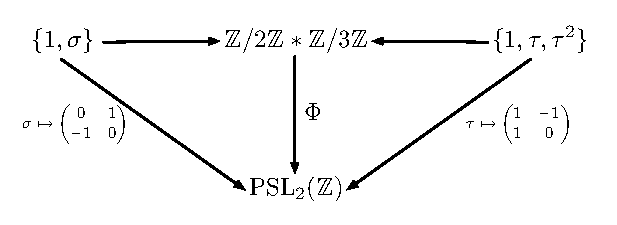
\includegraphics{grugraImages/PSL}
\end{center}
Der Nachweis, dass $\Phi$ in der Tat ein Isomorphismus ist, ist nicht
trivial.
\end{enumerate}

\BEM Die Konstruktion der freien Produkte lässt sich
ohne Weiteres auf beliebige Indexmengen $I$ verallgemeinern:
\begin{enumerate}
\item Es seien $(G_i)_{i\in I}$ Gruppen. Dann gibt es eine (bis auf
Isomorphie) eindeutige Gruppe $G=\AST_{i\in I} G_i$ und
Gruppenhomomorphismen $\alpha_i:G_i\Ra G$, so dass
für eine Gruppe $H$ und Homomorphismen $\phi_i:G_i\Ra H$
ein eindeutiger Homomorphismus $\Phi:G\Ra H$ existiert mit
$\Phi\circ\alpha_i=\phi_i$ für alle $i\in I$.
\item Ist $G_i=\lag S_i|R_i\rag$, so ist
$G=\lag \os{\bigcup}{.}_{i\in I}S_i|\os{\bigcup}{.}_{i\in I}R_i \rag$.
\item $G$ ist die Menge aller reduzierten Wörter über
$\os{\bigcup}{.}_{i\in I} G_i$, bei denen aufeinanderfolgende
Buchstaben aus verschiedenen $G_i$ kommen.
\end{enumerate}

\BEM\label{bem_freiprodukt}
Durch die Inklusionen
\begin{align*}
\iota_1:G_1\Ra G_1\times G_2,\quad g\mapsto(g,1) \\
\iota_2:G_2\Ra G_1\times G_2,\quad h\mapsto(1,h)
\end{align*}
ist über die UAE des freien Produktes ein Gruppenhomomorphismus
\[
\rho:G_1*G_2\Ra G_1\times G_2
\]
gegeben. Es gilt:
\begin{enumerate}
\item
\begin{align*}
\rho(g_1 h_1\cdots g_n h_n) &=
\rho(g_1)\rho(h_1)\cdots\rho(g_n)\rho(h_n) \\
&=\rho\circ\alpha_1(g_1)\rho\circ\alpha_2(h_1)\cdots\rho\circ\alpha_1(g_n)\rho\circ\alpha_2(h_n) \\
&=\iota_1(g_1)\iota_2(h_1)\cdots\iota_1(g_n)\iota_2(h_n) \\
&=(g_1,1)(1,h_1)\cdots(g_n,1)(1,h_n) \\
&=(g_1\cdots g_n,h_1\cdots h_n).
\end{align*}
\item $\rho$ ist surjektiv, also
\[
G_1\times G_2 \cong G_1*G_2/\K{\rho}.
\]
\item $\K{\rho}$ ist eine freie Gruppe mit Basis
\[
X=\{ ghg^{-1}h^{-1}:g\in G_1\backslash\{1\},h\in G_2\backslash\{1\}\}.
\]
\end{enumerate}
In Buch von Serre \cite{serre} wird ein elementarer Beweis hierfür
gebracht, den wir nun kurz skizzieren:
Zuerst rechnet man leicht nach, dass $K:=\lag X\rag$ ein Normalteiler
und im Kern von $\rho$ enthalten ist, d.h. es gibt ein $\tilde{\rho}$,
so dass
\[\xymatrix{
G_1*G_2 \ar[r]^{\rho}\ar[d] & G_1\times G_2 \\
G_1*G_2/K \ar[ur]_{\tilde{\rho}}
}\]
kommutiert. Zeigt man nun, dass $\tilde{\rho}$ ein Isomorphismus
(mit Umkehrabbildung $(g,h)\mapsto gh K$) ist, so folgt
$\K{\rho}=K$. Nun muss noch gezeigt werden, dass der Kern frei ist.

Später werden wir einen anderen Beweis für diese Bemerkung geben.

Über die Inklusionen $\iota_1$, $\iota_2$ fassen wir $G_1$ und $G_2$
als Untergruppen von $G_1*G_2$ mit $G_1\cap G_2=\{1\}$ auf.
Dies wollen wir im Folgenden verallgemeinern für Gruppen $G_1$, $G_2$,
$A$ mit $A\leq G_1$ und $A\leq G_2$. Gesucht ist eine Gruppe
$G_1 *_A G_2$ mit $G_1, G_2 \leq G_1 *_A G_2$ und
$G_1 \cap G_2 = A$.

\PROP\label{prop_AP}
Es seien $G_1$, $G_2$, $A$ Gruppen und $\alpha_i:A\Ra G_i$
Homomorphismen.
Dann gibt es eine Gruppe $G_1*_A G_2$ und Homomorphismen
$f_i:G_i\Ra G$ mit $f:=f_1\circ \alpha_1=f_2\circ\alpha_2$,
die folgende UAE erfüllt:
Für alle Gruppen $H$ und Homomorphismen $\phi_i:G_i\Ra H$ mit
$\phi_1\circ\alpha_1=\phi_2\circ\alpha_2$ gibt es genau einen
Homomorphismus $\Phi:G_1 *_A G_2 \Ra H$ mit $\Phi\circ f_i=\phi_i$,
d.h. das folgende Diagramm kommutiert:
\[\xymatrix{
& H & \\
G_1 \ar[r]^{f_1} \ar[ur]^{\phi_1} &
	G_1*_A G_2 \ar[u]_{\Phi} &
	G_2 \ar[l]_{f_2} \ar[ul]_{\phi_2}\\
& A \ar[ul]^{\alpha_1} \ar[ur]_{\alpha_2}  \ar[u]_{f}&
}\]
Wir nennen $G_1*_A G_2$ das \emph{amalgamierte Produkt}\index{amalgamiertes Produkt}\index{$G_1*_A G_2$}
von $G_1$ und $G_2$ über $A$.

\bew Die \textsl{Eindeutigkeit} folgt (wie immer bei einer UAE) wie
im Beweis zu Proposition \ref{prop_FP}.

Zur \textsl{Existenz} des amalgamierte Produktes:
Das Diagramm
\[\xymatrix{
G_1 \ar[r]^{\iota_1}  &
	G_1* G_2 &
	G_2 \ar[l]_{\iota_2}\\
& A \ar[ul]^{\alpha_1} \ar[ur]_{\alpha_2}  &
}\]
ist i.A. nicht kommutativ, da
$\iota_1\circ\alpha_1\neq\iota_2\circ\alpha_2$.
Wir entfernen den Teil, der die Kommutativität stört:
\[
N :=
\lag (\iota_1\circ\alpha_1(a))\cdot(\iota_2\circ\alpha_2(a))^{-1}
:a\in A \rag_{\mathrm{NT}}.
\]
Nun kommutiert der obere Teil des Diagramms
\[\xymatrix{
& (G_1*G_2)/N & \\
G_1 \ar[r]^{\iota_1} \ar[ur]^{f_1}  &
	G_1* G_2 \ar[u]_{p} &
	G_2 \ar[l]_{\iota_2} \ar[ul]_{f_2} \\
& A \ar[ul]^{\alpha_1} \ar[ur]_{\alpha_2}  &
}\]
dabei sei $p$ die kanonische Projektion. Definiere nun
\begin{align*}
G_1 *_A G_2 &:= (G_1*G_2)/N \\
f_i &:= p\circ \iota_i, \quad i=1,2.
\end{align*}
Es gilt nun
$f_1\circ\alpha_1(a) = f_2\circ\alpha_2(a)$ für alle $a\in A$,
also
\[
f_1\circ\alpha_1 = f_2\circ\alpha_2.
\]
Es bleibt zu zeigen, dass diese Konstruktion die UAE erfüllt:\\
Es seien $H,\phi_1,\phi_2$ wie gefordert. Wir nutzen die UAE
des freien Produkts, um einen eindeutigen Homomorphismus
$\hat{\Phi}:G_1*G_2\Ra H$ zu erhalten mit
$\hat{\Phi}\circ\iota_i=\phi_i$.
\[\xymatrix{
G_1 \ar[r]^{\iota_1} \ar[dr]_{\phi_1} &
	G_1 * G_2 \ar[d]_{\hat{\Phi}} &
	G_2 \ar[l]_{\iota_2} \ar[dl]^{\phi_2} \\
& H &
}\]
Für alle $a\in A$ gilt
\begin{align*}
\hat{\Phi}((\iota_1\circ\alpha_1(a))\cdot(\iota_2\circ\alpha_2(a))^{-1})
&= (\hat{\Phi}\circ\iota_1\circ\alpha_1(a))
\cdot (\hat{\Phi}\circ\iota_2\circ\alpha_2(a))^{-1} \\
&= (\phi_1\circ\alpha_1(a))\cdot(\phi_2\circ\alpha_2(a))^{-1} \\
&= 1 \qquad\text{(nach Voraussetzung)}
\end{align*}
und somit ist $N$ im Kern von $\hat{\Phi}$ enthalten.
Also gibt es einen eindeutigen Homomorphismus $\Phi$, der das
folgende Diagramm kommutativ macht
\[\xymatrix{
G_1 * G_2 \ar[d]_{p} \ar[r]^{\hat{\Phi}} & H \\
(G_1*G_2)/N \ar[ur]_{\Phi}
}\]
d.h. es ist $\Phi\circ p=\hat{\Phi}$.
Es gilt nun
$\Phi\circ f_i = \Phi\circ p\circ \iota_i=\hat{\Phi}\circ\iota_i
=\phi_i$.
\qed

\BEM Sei $I$ eine beliebige Indexmenge.
Wie beim freien Produkt lässt sich die Definition des
amalgamierten Produktes $\AST_{A,i\in I} G_i$ für Gruppen $A$, $G_i$
und Homomorphismen $\alpha_i:A\Ra G_i$ mit
$i\in I$ übertragen.

\BSP Amalgamierte Produkte.
\begin{enumerate}
\item Ist $A=\{1\}$, so ist $G_1*_A G_2=G_1*G_2$.
\item Ist $G_1*_A A=G_1$, so muss wegen der UAE $\alpha_2=\id$ 
gelten.
\item Ohne Beweis stellen wir fest:
Es ist $\ZZ/4\ZZ *_{\ZZ/3\ZZ} \ZZ/6\ZZ\cong\SL_2(\ZZ)$.
Die Gruppe $\SL_3(\ZZ)$ kann nicht als nichttriviales amalgamiertes
Produkt geschrieben werden.
\item Dieses Beispiel zeigt, dass das amalgamierte Produkt von
den $\alpha_i$ abhängt. Betrachte $\ZZ*_{\ZZ} \ZZ$
mit $\alpha_i=\id$.
Die UAE wird von $\ZZ*_{\ZZ} \ZZ=\ZZ$ erfüllt:
\[\xymatrix{
& \ZZ & \\
\ZZ \ar[ur]^{\id} & & \ZZ \ar[ul]_{\id} \\
& \ZZ \ar[ul]^{\id} \ar[ur]_{\id} &
}\]
Nun betrachte $\ZZ*_{\ZZ}\ZZ$ mit $\alpha_1(z)=2z$ und
$\alpha_2(z)=4z$.
\[\xymatrix{
& \ZZ*_{\ZZ}\ZZ & \\
\ZZ \ar[ur]^{f_1} & & \ZZ \ar[ul]_{f_2} \\
& \ZZ \ar[ul]^{z\mapsto 2z} \ar[ur]_{z\mapsto 4z} &
}\]
Angenommen, es wäre $\ZZ *_{\ZZ}\ZZ=\ZZ$. Dann gibt es
$f_1,f_2:\ZZ\Ra\ZZ$, so dass obiges Diagramm kommutativ ist.
Da $f_2$ als Homomorphismus $\ZZ\Ra\ZZ$ die Form $z\mapsto kz$
haben muss, ist wegen der Kommutativität $f_1$ durch
$z\mapsto 2kz$ gegeben.
Wählt man nun $H=\ZZ/2\ZZ$ und $\phi_1\neq 0$ und $\phi_2=0$,
so gibt es einen eindeutigen Homomorphismus $\Phi:\ZZ\Ra\ZZ/2\ZZ$
mit
\[
\bar{1} = \phi_1(1) = \Phi\circ f_1(1) = \Phi(2k) = \Phi \circ f_2(1)
\phi_2(1) = \bar{0}.
\]
Dies ist ein Widerspruch.
\item Es sei $G_1=\PSL_2(\QQ)$, $G_2=\ZZ/2\ZZ$ und $A=\ZZ$ und weiter
$\alpha_1:\ZZ\Ra \PSL_2(\QQ)$ ein beliebiger injektiver Homomorphismus
und $\alpha_2:\ZZ\Ra \ZZ/2\ZZ$, $z\mapsto z\mod 2$.
Dann ist
\[
\PSL_2(\QQ)*_{\ZZ} \ZZ/2\ZZ = \{ 0 \}.
\]
\[\xymatrix{
& H & \\
\PSL_2(\QQ) \ar[r]^{f_1} \ar[ur]^{\phi_1} &
	\{0\} \ar[u]_{0} &
	\ZZ/2\ZZ \ar[l]_{f_2} \ar[ul]_{\phi_2}\\
& \ZZ \ar[ul]^{\alpha_1} \ar[ur]_{\alpha_2} &
}\]
Um dies einzusehen, zeigen wir zunächst, dass für Homomorphismen
$\phi_1:\PSL_2(\QQ)\Ra H$ und $\phi_2:\ZZ/2\ZZ\Ra H$ mit
$\phi_1\circ\alpha_1=\phi_2\circ\alpha_2$ stets
$\phi_1=\phi_2=0$ gilt: Da $\alpha_2$ nicht injektiv ist, kann
auch $\phi_2\circ\alpha_2=\phi_1\circ\alpha_1$ nicht injektiv sein.
Da $\alpha_1$ injektiv ist, kann also $\phi_1$ nicht injektiv sein,
also ist $\K{\phi_1}\neq\{I_2\}$.
Da $\PSL_2(\QQ)$ eine einfache Gruppe ist (d.h. sie hat nur
$\{I_2\}$ und $\PSL_2(\QQ)$ selbst als Normalteiler) muss
$\K{\phi_1}=\PSL_2(\QQ)$ gelten, also $\phi_1=0$ und somit
auch $\phi_2\circ\alpha_2=0$. Da $\alpha_2$ surjektiv ist,
folgt $\phi_2=0$.

Die Nullabbildung $\{0\}\Ra H$ erfüllt also die UAE des amalgamierten
Produktes.
\end{enumerate}

Im Folgenden sei $I$ stets eine beliebige Indexmenge und
$G:=\AST_{A,i\in I} G_i$. Außerdem seien alle
$\alpha_i:A\Ra G_i$ injektiv.

\DB\
\begin{enumerate}
\item Es ist
\[
G = \AST_A G_i = (\AST G_i)/N
=\bigl\{x_1\cdots x_n : n\in\NN, x_j\in\BCUP{.}{i\in I} G_i \bigr\}.
\]
Diese Darstellung der Elemente ist i.A. nicht eindeutig.
Ist etwa $a\in A$, $g\in G_i$ und $h\in G_j$ mit $i\neq j$, so
ist stets
\[
(ga)hN = g(ah)N.
\]
\item Für jedes $i$ ist $A\leq G_i$. Es gibt also ein Vertretersystem
$S_i$ der Rechtsnebenklassen von $A$ in $G_i$, so
dass für jede Rechtsnebenklasse genau ein Repräsentant
in $S_i$ enthalten ist und $A$ selbst durch $1$ in $S_i$ repräsentiert
wird.
Dann kann jedes Element $x\in G$ eindeutig geschrieben werden
als
\[
x = as_1\cdots s_n N
\]
mit $a\in A$, $n\in\NN$ und $s_{\nu}\in S_{i_{\nu}}\backslash\{1\}$,
$i_{\nu}\neq i_{\nu+1}$.
Wir bezeichnen diese Darstellung als \emph{Normalform}\index{Normalform} von $x$.
\end{enumerate}
\textsc{Beweis von 2.:}
Setze
\[
X :=
\{ (a,s_1,\ldots,s_n): a\in A, n\in\NN,
s_{\nu}\in S_{i_{\nu}}\backslash\{1\},
i_{\nu}\neq i_{\nu+1} \}
\]
und
\[
\beta:X\Ra G,\quad (a,s_1,\ldots,s_n)\mapsto a s_1\cdots s_n N.
\]
$\beta$ ist offensichtlich surjektiv. Zu zeigen bleibt,
dass $\beta$ auch injektiv ist:\\
Setze
\[
Y_i :=
\{ (a,s_1,\ldots,s_n)\in X : a=1, s_1\not\in S_i \}.
\]
Dann ist die Abbildung
\[
X\Ra A\times S_i\times Y_i,\quad
(a,s_1,\ldots,s_n)\mapsto \left\{
\begin{matrix}
(a,s_i,(1,s_2,\ldots,s_n)), & s_1\in S_i \\
(a,1,(1,s_1,\ldots,s_n)), & s_1\not\in S_i
\end{matrix}
\right.
\]
bijektiv mit Umkehrung
\[
A\times S_i\times Y \Ra X,\quad
(a,s,(s_1,\ldots,s_n))\mapsto \left\{
\begin{matrix}
(a,s,s_1,\ldots,s_n), & s \neq 1 \\
(a,s_1,\ldots,s_n), & s = 1
\end{matrix}
\right..
\]
Da es auch eine Bijektion
$A\times S_i \Ra G_i$, $(a,s)\mapsto as$, gibt,
erhalten wir eine Bijektion
$\theta_i:X\Ra G_i\times Y_i$.
Da $G_i$ auf $G_i\times Y_i$ durch $g(g',y):=(gg',y)$ operiert,
induziert $\theta_i$ eine Aktion von $G_i$ auf $X$.
Wir erhalten für $a\in A\leq G_i$
\[
a(b,s_1,\ldots,s_n) = (ab,s_1,\ldots,s_n)\qquad (*)
\]
und für $s\in S_i\backslash\{1\}$, $x=(1,s_1,\ldots,s_n)\in X$ mit
$s_1\not\in S_i$
\[
s(1,s_1,\ldots,s_n) = (1,s,s_1,\ldots,s_n). \qquad (**)
\]
Nach $(*)$ ist die Aktion von $A$ auf $X$ unabhängig von der Wahl
der Einbettung in $G_i$. Daher liefert die UAE von $G$ eine
Operation von $G$ auf $X$ durch
\[
(x_1\cdots x_n N)\cdot x := x_1\cdots x_n x,\qquad x\in X, x_i\in G_i.
\]
Es sei $\alpha:G\Ra X$, $g\mapsto g (1)$.
Damit gilt für alle $(a,s_1,\ldots,s_n)\in X$:
\begin{align*}
\alpha\circ\beta(a,s_1,\ldots,s_n)
&= \alpha(a s_1\cdots s_n N) = a s_1\cdots s_n (1) \\
&\os{=}{(**)} a s_1\cdots s_{n-1}(1,s_n) \\
&\os{=}{(**)} \ldots \\
&\os{=}{(**)} a(1,s_1,\ldots,s_n) \\
&\os{=}{(*)} (a,s_1,\ldots,s_n).
\end{align*}
Folglich ist $\alpha\circ\beta=\id$ und $\beta$ injektiv.
\qed

\FOLG\
\begin{enumerate}
\item Sind $\alpha_1$ und $\alpha_2$ injektiv, so sind auch
$f_1$, $f_2$ und $f$ injektiv.
\item In $\AST_{A} G_i$ gilt $\BCAP{}{i\in I} G_i = A$.
\end{enumerate}
\bew
\begin{enumerate}
\item Wähle $g,g'\in G_1$ mit $f_1(g)=f_1(g')$.
Dann haben wir eindeutige Darstellungen $g=as$ und $g'=a's'$
und somit $gN=g'N$. Es folgt und $asN=a's'N$ und wegen der
Eindeutigkeit $a=a'$ und $s=s'$.
\item Angenommen es gibt ein $x\in \bigcap G_i$, $x\not\in A$.
Dann gibt es für alle $i$ eine eindeutige Darstellung
$x=a_i s_i$ mit $s_i\neq 1$.
Es folgt $xN=a_i s_i N$ für alle $i$.
Da alle $a_i$ gleich sein müssen, müssen auch alle $s_i$ gleich sein
und somit aus demselben $S_i$ stammen, im Widerspruch zur Annahme.
\qed
\end{enumerate}

Im Folgenden werden wir einfach $x_1\cdots x_n$ für
$x_1\cdots x_n N$ schreiben.


\DB\ \begin{enumerate}
\item Es sei $x=a s_1\cdots s_n \in G=\AST_A G_i$ in Normalform.
$\typ(x):=(i_1,\ldots,i_n)$ heißt \emph{Typ}\index{Typ} von $x$ und
$\ell(x):=n$ die \emph{Länge}\index{Länge} von $x$.
Typ und Länge sind unabhängig vom Vertretersystem.
\item Es ist $\ell(x)=0$ genau dann, wenn $x\in A$.
\item Es ist $\ell(x)\leq 1$ genau dann, wenn $x\in G_i$ für
ein $i$.
\item Es sei $\ell(x)\geq 2$. Dann heißt $x$ \emph{zyklisch reduziert}\index{zyklisch reduziert},
wenn $i_1\neq i_n$.
\item Jedes $x\in G$ ist konjugiert zu einem zyklisch reduzierten
Element oder zu einem Element, dass bereits in einem $G_i$ enthalten
ist.
\item Jedes zyklisch reduzierte Element hat unendliche Ordnung.
\item Jedes $x\in G$ von endlicher Ordnung ist konjugiert zu
einem Element aus einem der $G_i$.
\item Sind alle $G_i$ torsionsfrei (d.h. sie enthalten keine Elemente
endlicher Ordnung), so ist auch $G$ torsionsfrei.
\end{enumerate}
\bew 7. und 8. folgen direkt aus 5. und 6. .
\begin{enumerate}
\item[5.] Es sei $n\geq 2$ und $x$ nicht zyklisch reduziert.
Es ist
\begin{align*}
s_n x s_n^{-1}
&= \ub{s_n a s_1}{\in G_{i_1}} s_2\cdots s_{n-1} \\
&= a's' s_2\cdots s_{n-1}
\end{align*}
mit geeigneten $a'\in A$, $s'\in S_{i_1}$.
Es ist $\ell(a's's_2\cdots s_{n-1})<\ell(x)$.
Mit Induktion folgt die Behauptung.
\item[6.] Es sei $x=a s_1\cdots s_n$ in Normalform mit $\ell(x)\geq 2$
und $i_1\neq i_n$.
Wiederholtes bilden der Normalform liefert:
\begin{align*}
x^2 &= a s_1 \cdots \ub{s_n a}{=a' s_n'} s_1 \cdots s_n \\
&= a s_1 \cdots \ub{s_{n-1} a'}{=a'' s_{n-1}'} s_n' s_1\cdots s_n \\
&= \ldots\\
&= \tilde{a} s_1' \cdots s_n' s_1 \cdots s_n
\end{align*}
für geeignete $\tilde{a},a',a'',\ldots\in A$ und
$s_{\nu}'\in S_{i_{\nu}}$.
Der letzte Ausdruck ist die Normalform von $x^2$, da $s_n'$ und $s_1$
aus verschiedenen $S_{i_{\nu}}$ stammen.
Es folgt nun $\ell(x^2)=2\ell(x)$,
$\typ(x^2)=(i_1,\ldots,i_n,i_1,\ldots,i_n)$.
Induktiv erhalten wir $\ell(x^k)=k\ell(x)$,
also $x^k\neq 1$ für alle $k\geq 1$.
\qed
\end{enumerate}

%======================
\section{Graphen von Gruppen}\label{sec_GvG}

\DB Es sei $G$ eine Gruppe, $\GR$ ein Graph und
$\rho:G\Ra\Aut(\GR)$ eine Aktion von $G$ auf $\GR$.
Wir schreiben $gx:=\rho(g)_E(x)$ und $gk:=\rho(g)_K(k)$.
\begin{enumerate}
\item Für $x\in E(\GR)$ sei
\[
G_x := \{ g\in G : gx = x \}
\]
die \emph{Fixgruppe}\index{Fixgruppe}\index{Gruppe!Fix-}\index{$G_x$}
von $x$.
Entsprechend ist $G_k$ für $k\in K(\GR)$ definiert.
\item Für alle $g\in G$ und $x\in E(\GR)$ gilt
\[
G_{gx} = g G_x g^{-1},
\]
und enstprechendes für $G_{gk}$, $k\in K(\GR)$.
\item Für jede Kante $k\in K(\GR)$ gilt
\[
G_k \leq G_{\ini(k)}\cap G_{\ter(k)}.
\]
\end{enumerate}
\bew \begin{enumerate}
\item[2.] Es ist $h(gx)=gx$ genau dann, wenn $(g^{-1} h g)x=x$ gilt.
Es ist also $h\in G_{gx}$ genau dann, wenn $g^{-1}hg\in G_x$ gilt,
und dies ist wiederum äquivlent zu $h\in gG_x g^{-1}$.
\item[3.] Klar.
\qed
\end{enumerate}

\PROP Jede inversionsfreie Aktion $\rho:G\Ra\Aut(\GR)$ bestimmt
folgende Daten:
\begin{itemize}
\item Einen Graphen $\bar{\GR}:= \GR/G$.
\item Für jede Ecke $x\in E(\bar{\GR})$ eine Gruppe $G_x$, nämlich
$G_x := G_{\tilde{x}}$ für ein Urbild $\tilde{x}\in E(\GR)$ von $x$.
\item Für jede Kante $k\in K(\bar{\GR})$ eine Gruppe $G_k$, nämlich
$G_k := G_{\tilde{k}}$ für ein Urbild $\tilde{k}\in K(\GR)$ von $k$.
Dabei ist $G_{\bar{k}}=G_k$ für die Gegenkante $\bar{k}$.
\item Für jede Kante $k$ einen injektiven Gruppenhomomorphismus
$\alpha_k:G_k\Ra G_{\ini(k)}$
(durch $G_{\tilde{k}}\hookrightarrow G_{\ini(\tilde{k})}$).
Beachte: $\alpha_{\bar{k}}:G_k\Ra G_{\ter(k)}$.
\end{itemize}
Ein solches Tupel $(\bar{\GR}, G_x, G_k, \alpha_k)$ heißt
\emph{Graph von Gruppen}\index{Graph!von Gruppen}.

\BSP Graphen von Gruppen.
\begin{enumerate}
\item Ist $\rho$ eine freie Aktion, so ist $G_x=G_k=\{1\}$ für
alle $x\in E$, $k\in K$.
\item Es sei $\GR$ die unendliche lineare Kette
\begin{center}
	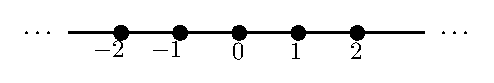
\includegraphics{cay1}
\end{center}
und $G=\Aut(\GR)$ wird erzeugt von der Translation $t$ um $1$ und
der Spiegelung $s$ an der $0$. Die Aktion von $G$ auf $\GR$ ist nicht
inversionsfrei. $G$ operiert jedoch inversionsfrei auf
der baryzentrischen Unterteilung
\begin{center}
	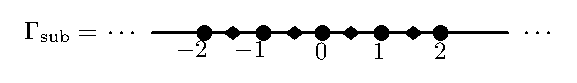
\includegraphics{cay1sub}
\end{center}
Es ist
\begin{center}
	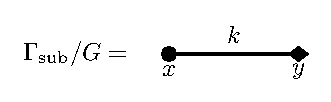
\includegraphics{cay1subquot}
\end{center}
und $G_x=\ZZ/2\ZZ$, $G_y=\ZZ/2\ZZ$, $G_k=\{1\}$.
Der entsprechende Graph von Gruppen ist
\begin{center}
	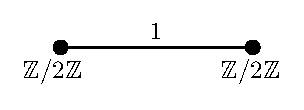
\includegraphics{GvG1}
\end{center}
Wir werden später sehen, dass $G\cong \ZZ/2\ZZ*\ZZ/2\ZZ$ gilt.
\item $G=\SL_2(\ZZ)$ wird erzeugt von
\[
T=\begin{pmatrix}
1 & 1 \\ 0 & 1
\end{pmatrix},\quad
S=\begin{pmatrix}
0 & -1 \\ 1 & 0
\end{pmatrix}.
\]
Es ist $\ord(T)=\infty$ und $\ord(S)=4$.
Die Gruppe $\SL_2(\ZZ)$ operiert auf der komplexen oberen Halbebene\index{obere Halbebene}\index{Halbebene}
\[
\hh = \{ z\in\CC : \Im(z) > 0 \}.
\]
Die Aktion ist für
$A=\begin{pmatrix} a&b \\ c&d \end{pmatrix}\in \SL_2(\ZZ)$
und $z\in \hh$ definiert durch die \emph{Möbiustransformation}\index{Möbiustransformation}
\[
A\cdot z := \frac{az+b}{cz+d},
\]
insbesondere gilt $T\cdot z= z+1$ und $S\cdot z=-\frac{1}{z}$.
Wir betrachten nun zunächst den \emph{Fundamentalbereich}\index{Fundamentalbereich}
\[
F = \Bigl\{ z\in \hh : -\frac{1}{2}\leq \Re(z) \leq \frac{1}{2},
|z| \geq 1 \Bigr\}
\]
in $\hh$.
\begin{center}
	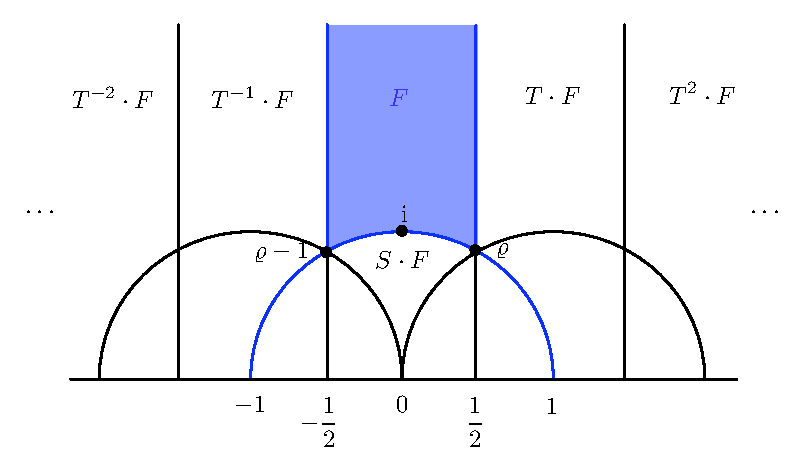
\includegraphics{fundbereich}
\end{center}
Alle $z\in \hh$ können durch wiederholte Aktion von $T$ und $S$
in den Fundamentalbereich $F$ bewegt werden.
Es bezeichne $R_{\rho}$ das Kreissegment, das von
$\rho$ durch $\i$ nach $\rho-1$ läuft:
\begin{center}
	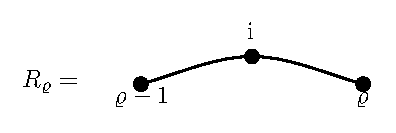
\includegraphics{rho}
\end{center}
$\SL_2(\ZZ)$ operiert auf dem Baum
\[
\GR := \BCUP{}{A\in\SL_2(\ZZ)} A\cdot R_{\rho}.
\]
Der Quotientengraph ist
\begin{center}
	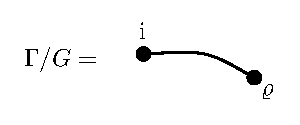
\includegraphics{rhoquot}
\end{center}
Es ist $G_{\i}=\lag S\rag \cong \ZZ/4\ZZ$,
$G_{\rho}=\lag TS\rag\cong \ZZ/6\ZZ$ und
$G_k=\lag I_2\rag \cong\ZZ/2\ZZ$.
Die Abbildung $\alpha_k$ ist durch $\alpha_k(-I_2)=S^2$ und
$\alpha_{\bar{k}}$ durch
$\alpha_{\bar{k}}(-I_2)=(TS)^3$ gegeben.
Aus Beispiel \ref{bsp_amprod}(3) wissen wir bereits,
dass $\SL_2(\ZZ)\cong \ZZ/4\ZZ*_{\ZZ/2\ZZ} \ZZ/6\ZZ$ ist.
\end{enumerate}
